\documentclass[letter, 10pt]{report}

\usepackage[utf8]{inputenc}
\usepackage[T1]{fontenc}
\usepackage[french]{babel} 
\usepackage{graphicx}
%\usepackage{url} %pour écrire des adresses cliquables
%\usepackage{lmodern} %pour changer le pack de police
%\usepackage[top=5cm, bottom=5cm, left=6cm, right=3cm]{geometry} %pour les marges
\usepackage[usenames, dvipsnames]{color}
\usepackage{listings}
\usepackage{hyperref} %pour un fichier PDF  interactif

\pdfcompresslevel=9

\hypersetup{
	backref=true, %permet d'ajouter des liens dans...
	pagebackref=true, %...les bibliographies
	hyperindex=true, %ajoute des liens dans les index.
	colorlinks=true, %colorise les liens
	breaklinks=true, %permet le retour à la ligne dans les liens trop longs
	urlcolor=blue, %couleur des hyperliens
	linkcolor=blue, %couleur des liens internes
	bookmarks=true, %créé des signets pour Acrobat
	bookmarksopen=true,%si les signets Acrobat sont créés,
	%les afficher complètement.
	%pdftitle={Mon fabuleux livre}, %informations apparaissant dans
	%pdfauthor={Pejvan BEIGUI},%dans les informations du document
	%pdfsubject={Mac OS X}%sous Acrobat.
}


\lstdefinestyle{php}{
	language=PHP,
	caption={PHP},
	basicstyle= \footnotesize,
	tabsize=4,
	showspaces=false,
	showstringspaces=false,
	showtabs=false,
	breaklines=true,
	breakautoindent=true,
	identifierstyle=\color{RoyalBlue},
	commentstyle=\color{LimeGreen},
	keywordstyle=\color{Black},
	stringstyle=\color{OrangeRed},
	backgroundcolor=\color{white},
	numbers=left
}

\title{Carcajou}
\author{\textsc{Martin Desharnais} \\ \textsc{Samuel Milette-Lacombe} \\ \textsc{Marc-André Destrempes}}
\date{\today}

\begin{document}

\maketitle

\begin{abstract}
Ce document contient la documentation du projet de médiathèque (nom de code «~Carcajou~») conçu pour le département de musique du cégep de Trois-Rivières.
\end{abstract}

\newpage
\tableofcontents
\newpage

%%%%%%%%%%%%%%%%%%%%%%%%%%%%%%%%%%%%%%%%%%%%%%%%%%
\chapter{Spécifications fonctionnelles}
%%%%%%%%%%%%%%%%%%%%%%%%%%%%%%%%%%%%%%%%%%%%%%%%%%

\section{Caractéristiques}

%%%%%%%%%%%%%%%%%%%%%%%%%%%%%%%%%%%%%%%%%%%%%%%%%%
\chapter{Architecture du système}
%%%%%%%%%%%%%%%%%%%%%%%%%%%%%%%%%%%%%%%%%%%%%%%%%%

\section{Maquette et charte graphique}
\section{Modèle des pages principales et secondaires}
\section{Diagramme d'enchaînement}
\section{Diagramme de classe}
\section{Base de données et dictionnaire}

%%%%%%%%%%%%%%%%%%%%%%%%%%%%%%%%%%%%%%%%%%%%%%%%%%
\chapter{Architecture technologique}
%%%%%%%%%%%%%%%%%%%%%%%%%%%%%%%%%%%%%%%%%%%%%%%%%%

\section{Représentation graphique}
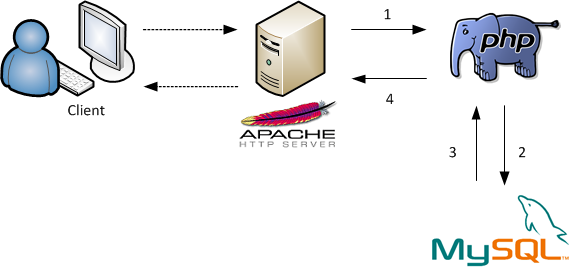
\includegraphics[scale=0.7]{architectureTechnologique.png}

\section{Spécifications techniques}

\subsection{Navigateurs}
Lors de la conception le site à été testé sur les navigateurs suivants:

\begin{itemize}
\item Mozilla Firefox 3.5.16
\item Mozilla Firefox 4.0.1
\item Google Chrome 6.0.472.63
\item Google Chrome 11.0.696.65
\end{itemize}

Le site est fonctionnel sur l'ensemble des navigateurs mais certains effets graphiques ne sont disponnibles que sur les versions récentes des navigateurs.

\subsection{Languages}
\subsubsection{Client}
Du coté client, les languages utilisés sont le HTML 5, le CSS3, le XML et le javascript. Pour ce qui est de l'utilisation du javascript, il a été décidé minimiser au maximum la dépendance du site.
Javascript avec utilisation de la bibliothèque jQuery 1.6.1
\subsubsection{Serveur}
PHP 5.3.3 -- 5.3.5

\subsection{Bande passante}
What the fuck?!?

\subsection{Serveurs}
\subsubsection{HTTP}
Apache HTTP Server 2.2.16 -- 2.2.17
\subsubsection{SGBD}
MySQL 5.1.49 -- 5.5.8

\subsection{Type de base de données}

\section{Sécurité}

La sécurité repose essentiellement sur la validation des droits des utilisateurs avant de générer les pages du site. C'est le PHP qui est chargé de valider que l'utilisateur courant dispose des droits suffisants avant d'ajouter une section à la page que le serveur HTTP s’apprête à retourner.

En pratique cela se traduit par un appel à la fonction application->currentUser->haveRights() en lui spécifiant en premier paramètre la section dont l'on veut tester les droits et en second paramètre la liste des droits dont l'utilisateur doit disposer pour avoir accès à ce contenu. Ces droits sont définis dans le tableau application->rights. Par exemple afin de valider que l'utilisateur à bien le droit d'accéder à la zone d'administration, il suffit d'utiliser le code suivant~:

\begin{lstlisting}[style=php]
if($application->currentUser->haveRights('administration', $application->rights['read'] | $application->rights['write']))
{
	// We can now print administration section
}
else
{
	// Current user does not have suffisent rights to se this section
}
\end{lstlisting}

%%%%%%%%%%%%%%%%%%%%%%%%%%%%%%%%%%%%%%%%%%%%%%%%%%
\chapter{Prototype fonctionnel}
%%%%%%%%%%%%%%%%%%%%%%%%%%%%%%%%%%%%%%%%%%%%%%%%%%

\end{document}
